\documentclass[10pt]{beamer}

% \usepackage[a4paper, left=0.6in, right=0.6in, top=0.85in, bottom=0.85in]{geometry}
\usepackage[utf8]{inputenc}
\usepackage{textcomp}
\usepackage{fontspec}
\usepackage[russian]{babel}
%\usepackage{polyglossia}
%\setdefaultlanguage[spelling=modern]{russian}
%\setotherlanguage{english}
\setmainfont{CMU Serif}
\setsansfont{CMU Sans Serif}
\setmonofont{CMU Typewriter Text}

\usepackage{amsmath, amssymb, amsthm, mathtools, thmtools, mathdots}

\newcommand\NN{\ensuremath{\mathbb{N}}}
\newcommand\RR{\ensuremath{\mathbb{R}}}
\newcommand\ZZ{\ensuremath{\mathbb{Z}}}
\renewcommand\O{\ensuremath{\varnothing}}
\newcommand\QQ{\ensuremath{\mathbb{Q}}}
\newcommand\CC{\ensuremath{\mathbb{C}}}

\theoremstyle{definition}

\newtheorem{lemmaf}{Лемма}
\newtheorem{theoremf}{Теорема}
\newtheorem{definitionf}{Определение}
\newtheorem{remark}{Замечание}
\newtheorem{statementf}{Утверждение}
\newtheorem{propositionf}{Предложение}

\newtheorem*{lemmaf*}{Лемма}
\newtheorem*{theoremf*}{Теорема}
\newtheorem*{remark*}{Замечание}
\newtheorem*{statementf*}{Утверждение}
\newtheorem*{propositionf*}{Предложение}

\usepackage{enumitem}
\usepackage{mleftright}
\usepackage{environ}
\usepackage{csquotes}

\NewEnviron{pArray}[1]
{
\left(\begin{array}{#1}
\BODY
\end{array}\right)
}
\usetheme{Madrid}
% \title{Необычная задача кубического представления}
% \author{Алексей Кислицын, Всеволод Триль, Андрей Владимиров}

\title{Необычная задача кубического представления}
\author{Алексей Кислицын \hspace{1mm} Андрей Владимиров \hspace{1mm} Всеволод Триль}
\institute{Механико-математический факультет МГУ}
\setbeamertemplate{footline}{}
\setbeamertemplate{footline}[frame number]{}
% \setbeamertemplate{theorems}[numbered]
\usepackage{animate}

\begin{document}
    
    \frame{\titlepage}

    \begin{frame}

        \onslide<+->{
        \begin{block}{Постановка задачи}
            Всё началось с, кажущейся на первый взгляд, детской задачки:
            
            \begin{figure}[H]
                \centering
                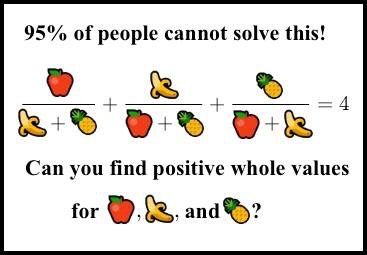
\includegraphics[width = 6cm]{../images/banana.jpg}
            \end{figure}
        \end{block}
        }

        \onslide<+->{
        \begin{block}{}
            В этом докладе мы предъявим алгоритм решения данной задачи, а также
            постараемся её обобщить и проанализировать.
        \end{block}
        }
    \end{frame}

    \begin{frame}
        \onslide<+->{
        \begin{block}{}
            Переформулируем ей в математических терминах: требуется найти все
            натуральные решения следующего уравнения при \(N = 4\):
            \[
                \frac{x}{y + z}  + \frac{y}{x + z} + \frac{z}{x + y} = N,
                \qquad x, y, z \in \NN
            .\]
            Мы пока не будем придавать значения тому, что \(N = 4\), а сразу
            будем рассматривать постановку задачи для произвольного \(N \in
            \NN\).
        \end{block}
        }

        \onslide<+->{
        \begin{block}{}
            Заметим, что решение исходного уравнения равносильно
            нахождению натуральных точек на кубике, заданной в однородных
            координатах \((x : y : z)\) следующим уравнением: 
            \[
                x^3 + y^3 + z^3 + (1 - N) (x^2 y + y^2 x + x^2 z + z^2 x + y^2 z + z^2 y)
                + (3 - 2 N) x y z = 0
            .\]
        \end{block}
        }
        
        \onslide<+->{
        \begin{block}{}
            Сразу отметим, что так как мы работаем в проективных координатах,
            то это равносильно нахождению точек с рациональными координатами,
            у которых знаки одинаковы.
        \end{block}
        }

        \onslide<+->{
        \begin{block}{}
            Но перед тем, как перейти к решению исходной задачи, рассмотрим более простую
            задачу -- поиск натуральных точек на квадрике 
        \end{block}
        }
    \end{frame}


    \begin{frame}
    \onslide<+->{
        \begin{block}{Описание рациональных точек на квадрике}
        	\begin{align}
        	a x^2 + b y^2 + c z^2 + d x y + e y z + f x z = 0,  \qquad a, b, c, d, e, f \in
        	\mathbb{Z} 
        	\end{align}
       
       
        \end{block}
    	
    	\begin{block}{Метод секущих}
    		Для начала заметим, что зная одну рациональную точку на квадрике можно получить все методом секущих. (картинка)
    	\end{block}
	}    
    \end{frame}
	
	
	\begin{frame}
		\onslide<+->{
			\begin{block}{Поиск рациональной точки. Шаг 1.}
			Приведем квадрику рациональным преобразованием к одному из следующих видов.
			\begin{align*}
			x^2 - A z^2 &= 0 \\
			x^2 - A y z &= 0 \\
			A x^2 + B y^2 - C z^2 &= 0 
			\end{align*}
			\end{block}
			
			\begin{block}{Шаг 2.}
				Случаи 1 и 2 разбираются тривиально. В третьим случае используем критерий Лежандра,  согласно нему уравнение 3 имеет целочисленное
				решение тогда и только тогда когда \(BC\) квадратичный вычет по модулю \(A\),
				\(AC\) - по модулю \(B\) и \(-AB\)  по модулю \(C\).
			\end{block}
			
			\begin{block}{Замечание}
				Таким образом поиск рациональной точки это полностью решенная проблема в случае квадрики. Более того есть теорема Хольцера, которая дает верхнюю оценку на границы в которых его надо искать.
			\end{block}
	}
	\end{frame}    

    \begin{frame}
        \onslide<+->{
        \begin{block}{Приведение к нормальной форме Вейерштрасса}
            Перейдём к основной задаче, как и в случае квадрики приведём кубику 
            \[
                x^3 + y^3 + z^3 + (1 - N) (x^2 y + y^2 x + x^2 z + z^2 x + y^2
                z + z^2 y) + (3 - 2 N) x y z = 0
            \] 
            к наиболее простому виду -- нормальной форме Вейерштрасса, которая
             может записывается так:
            \[
            y^2 z = x^3 + a x z^2 + b z^3, \quad a, b \in \CC
            .\]
        \end{block}
        }

        \onslide<+->{
        \begin{block}{}
            В нашем случае, так как коэффициенты кубики целые и проективные
            преобразования будут с целыми коэффициентами, то \(a, b \in \ZZ\).

            Далее, под проективными преобразованиями мы будем
            понимать только целочисленные проективные преобразования.
        \end{block}
        }

        \onslide<+->{
        \begin{block}{}
            Мы предъявим алгоритм приведения кубики к нормальной форме
            Вейерштрасса для произвольной кубики с целыми(рациональными)
            коэффициентами. 
        \end{block}
        }

    \end{frame}


    \begin{frame}
        \onslide<+->{
        \begin{block}{Шаг 0. Нахождение рациональных точек перегиба}
            Итак, пусть у нас есть кубика, заданная уравнением \(F(x, y, z) =
            0\), где 
            \begin{multline*}
            F(x, y, z) = a_{30} x^3 + a_{03} y^3 + a_{00} z^3 + a_{01} y z^2 + a_{10} x z^2 +
            a_{11} x y z + \\ + a_{21} x^2 y +
            a_{12} x y^2 + a_{20} x^2 z + a_{02} y^2 z
            ,\end{multline*}
            то есть \(a_{ij} \in \ZZ\) -- коэффициент при мономе \(x^{i} y^{j} z^{3 - i -
            j}\). 
        \end{block}
        }
    
        \onslide<+->{
        \begin{definitionf}
            Точка \(P_0\) кубики \(F(x^{1}, x^{2}, x^{3}) = 0\) называется
            \textit{точкой перегиба}, если касательная к ней в точке \(P\)
            имеет касание третьего порядка, то есть для любой точки \(Q =
            (x^{1}_q : x^{2}_q : x^{3}_q)\) на касательной выполнено
            \[
            \sum_{i,j = 1}^{3} \frac{\partial^2 F}{\partial x^{i} \partial
            x^{j}} (P_0) \, x^{i}_q x^{j}_q = 0
            .\] 
        \end{definitionf}
        }

    \end{frame}

    \begin{frame}
        \onslide<+->{
        \begin{definitionf}
            \textit{Гессианом} кубики \(F(x^{1}, x^{2}, x^{3}) = 0\) называется кубика
            \[
            H(F) := \det \left( \frac{\partial^2 F}{\partial x^{i} \partial
            x^{j}}\right)_{ij}
            .\] 
        \end{definitionf}
        }

        \onslide<+->{
        \begin{theoremf}
            Точки перегиба неособой кубики в \(\CC \mathrm{P}^2\) -- в точности
            точки пересечения кубики с её Гессианом.
        \end{theoremf}
        }

    \end{frame}

    \begin{frame}
        \onslide<+->{
        \begin{block}{}
            Мы не будем проверять кубику на наличие особенностей, а просто найдём
            все точки пересечения с Гессианом и посмотрим, есть ли там
            особенности. Если среди общих точек есть неособая, то нам эта точка
            подходит и мы можем переходить к следующему шагу. Если все точки
            особые, то алгоритм продолжить нельзя.
        \end{block}
        }

        
        \onslide<+->{
        \begin{block}{}
            Для поиска общих точек рассмотрим результант \(R(F, H(F))\) по
            переменной \(z\). Получим однородный многочлен 9-той степени.
            (дописать уточнение) Находим все его рациональный корни -- пары
            \((x, y)\) и подставляем в \(F\) и в \(H(F)\) для нахождения общей
            точки (или удостоверении, что при данных \((x_0, y_0)\) её нет).
        \end{block}
        }

        \onslide<+->{
        \begin{block}{}
            Этот шаг реализован в файле \textsf{InflectionPoints.py} в функции
            \textsf{find\_non\_singular\_inflection\_point}.
        \end{block}
        }
    \end{frame}

    \begin{frame}
        \onslide<+->{
        \begin{block}{Шаг 1. Избавление от монома \(y^3\)}
            Выберем какую-то рациональную точку перегиба \(P\) и переведём её в точку
            \((0 : 1 : 0)\) некоторым проективным преобразованием. После проективного
            преобразования, наша кубика имеет уравнение \(\widetilde{F}(\widetilde{x},
            \widetilde{y}, \widetilde{z})\), в котором нет \(\widetilde{y}\).
            Таким образом, у нас уйдёт моном \(y^3\).
        \end{block}
        }

        \onslide<+->{
        \begin{block}{}
            Этот шаг реализован в файле \textsf{WeierstrassForm.py} в функции
            \textsf{weierstrass\_form\_step1}.
        \end{block}
        }
    \end{frame}
    
    \begin{frame}
        \onslide<+->{
        \begin{block}{Шаг 2. Избавление от мономов \(y^2 x\) и \(y x^2\)}
            Теперь мы хотим сделать преобразование,
            сохраняющее точку \(O = (0 : 1 : 0)\), так, чтобы
            прямая \(z = 0\) была касательной к кубике \(\widetilde{F}\) в точке
            \(O\), то есть сделать преобразование \((\widetilde{x} :
            \widetilde{y} : \widetilde{z}) \to (x' : y' : z')\), такое что
            для \(F'(x', y', z')\) будет выполнено: 
             \[
            \frac{\partial F'}{\partial x'} (O) = \frac{\partial F'}{\partial y'}
            (O) = 0, \quad \frac{\partial F'}{\partial z'} (O) \ne 0
            .\]
            То есть нет монома \(x y^2\), однако, коэффициент при \(y^2 z\) отличен от
            нуля, и поэтому, разделив на него, можем считать, что он равен \(1\).
            Кроме того, так как \(O\) -- точка перегиба, то касание прямой \(z = 0\) с
            нашей кубикой имеет порядок 3, таким образом нет монома \(x^2 y\). 
        \end{block}
        }

    \end{frame}
    
    \begin{frame}
        \onslide<+->{
        \begin{block}{Шаг 3. Выделение \(y^2 z\) и избавление от \(x^2 z\)}
            После второго преобразования, уравнение нашей кубики стало \(F'(x', y',
            z') = 0\), где 
            \begin{multline*}
            F'(x', y', z') = a_{30}' \left( x' \right)^3 + a_{20}' \left( x' \right)^2
            z' + a_{11}' x' y' z' + \left( y' \right)^2 z' + \\
            + a_{10}' x' \left(
            z' \right)^2 + a_{01}' y' \left( z' \right)^2 + a_{00}' \left( z'
            \right)^3
            .\end{multline*}
        \end{block}
        }

        \onslide<+->{
        \begin{block}{}
            Делая замену \(y'' =  y' + (a_{01}' z' + a_{11}'
            x')/2\), выделяем полный квадрат по \(y'\) и уравнение кубики
            становится:
            \[
            \left( y'' \right)^2 z' = a_{30}'' \left( x' \right)^3 + a_{20}'' \left( x' \right)^2
            z' + a_{10}'' x' \left( z' \right)^2 + a_{00}'' \left( z' \right)^3
            .\] 
        \end{block}
        }

        \onslide<+->{
        \begin{block}{}
            Теперь линейной заменой \(x'' = x' - \dfrac{a_{20}''}{3 a_{30}''}
            z'\) избавляемся от монома \(\left( x' \right)^2 z'\) и получаем:
            \[
            \left( y'' \right)^2 z' = a_{30}''' \left( x'' \right)^3 + a_{10}''' x''
            \left( z' \right)^2 + a_{00}''' \left( z' \right)^3
            .\] 
        \end{block}
        }

    \end{frame}

    \begin{frame}
        \onslide<+->{
        \begin{block}{}
            Далее, делаем замену \(z'' = \dfrac{1}{a_{30}'''} z'\) и получаем:
            \[
            \left( y'' \right)^2 z'' = \left( x'' \right)^3 + a_{30}''' a_{10}''' x''
            \left( z'' \right)^2 + a_{00}''' \left( a_{30}''' \right)^2 \left( z'' \right)^3
            .\] 
            Обозначая \(a := a_{30}''' a_{10}''', b := a_{00}''' \left( a_{30}'''
            \right)^2\), получаем требуемую форму: 
            \[
            \left( y'' \right)^2 z'' = \left( x'' \right)^3 + a x''
            \left( z'' \right)^2 + b \left( z'' \right)^3
            .\] 
        \end{block}
        }
    
        \onslide<+->{
        \begin{remark*}
            Отметим, что все коэффициенты в ходе алгоритма получались
            целочисленными или рациональными (так как совершались только
            целочисленные проективные преобразования). Соответственно, если
            коэффициенты \(a, b\) оказались рациональными, мы их можем сделать
            целыми с помощью замены \(x''' = \dfrac{1}{d} x'', z''' = \dfrac{1}{d^3}
            z''\), где \(d\) -- наименьшее общее кратное знаменателей \(a, b\).
        \end{remark*}
        }
    \end{frame}

    \begin{frame}
		\onslide<+->{
        \begin{block}{}
            Опишем рациональные точки на кубике в форме Вейерштрасса.
            Пусть нам известно несколько точек, можно ли по ним как в
            случае квадрики получить ещё?
        \end{block}
        }

		\onslide<+->{
        \begin{block}{Сложение точек}
            
            
        \end{block}
        }

		\onslide<+->{
        \begin{figure}[H]

        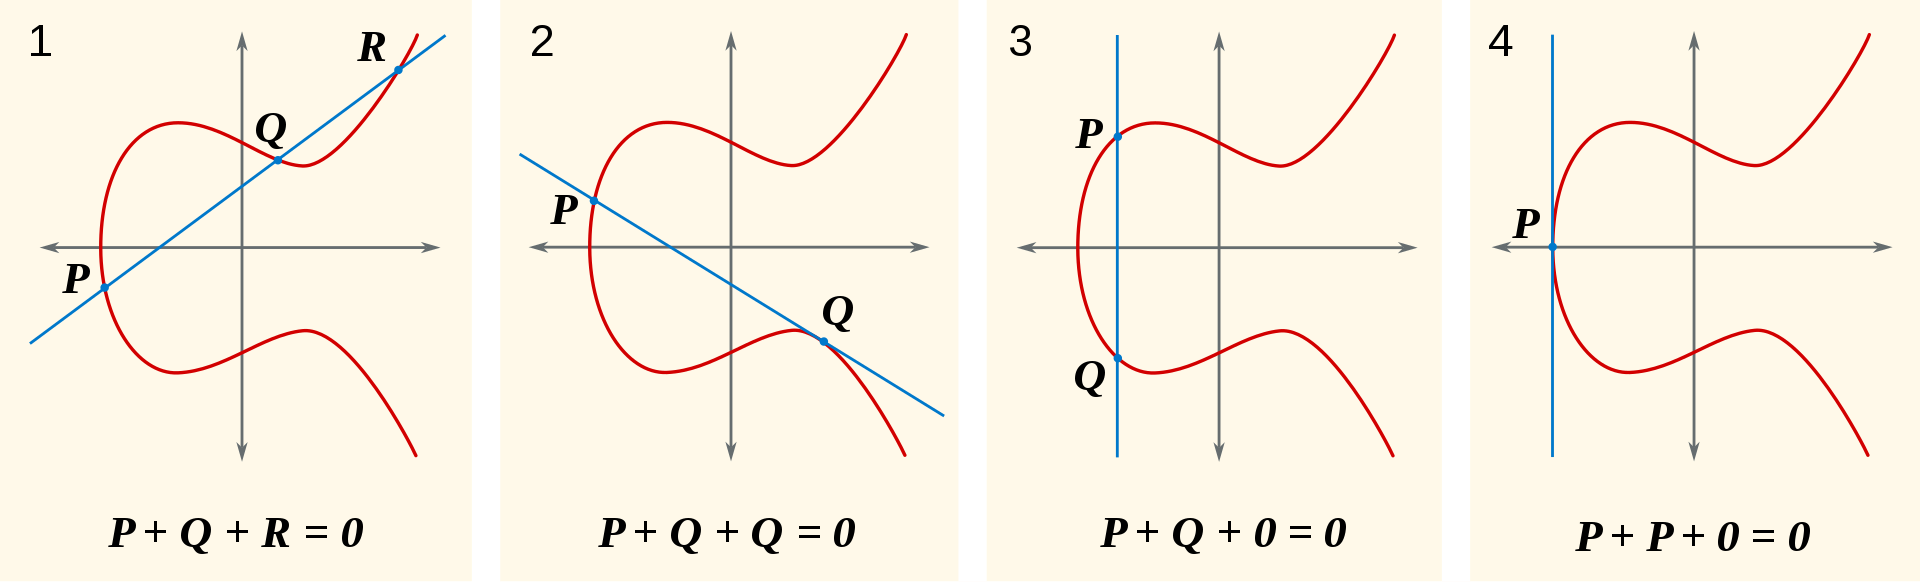
\includegraphics[width = 10cm]{../images/add2.png}
        \end{figure}
        }

		\onslide<+->{
        \begin{definitionf}
            Суммой точек \(P\) и \(Q\) назовём точку пересечения прямой \(PQ\) с
            кубикой, отражённую относительно оси \(x\) и будем обозначать \(P +
            Q\).
        \end{definitionf}
        }
	\end{frame}

	\begin{frame}
		\onslide<+->{
        \begin{theoremf}
            Множество рациональных точек кубики \(E(\QQ)\) в нормальной
            форме Вейерштрасса образуют абелеву группу. 
        \end{theoremf}
        }
    
        \onslide<+->{
        \begin{theoremf}[Морде]
            Группа \(E(\QQ)\) конечно порождена.
        \end{theoremf}
        }
		
        \onslide<+->{
        \begin{block}{}
            Это даёт надежду на полное описание рациональных точек на кубике.
            Ведь есть явные формулы для сложения точек в нормальной форме.
        \end{block}
		}
	\end{frame}


	\begin{frame}
		\onslide<+->{
		\begin{block}{Явные формулы для $P + Q$}
			Пусть \(P = (x_{p}, y_{p}), Q = (x_{q}, y_{q}), R =
			(x_{r}, y_{r})\), где \(R = P + Q\) и \(P \neq Q\). Тогда мы имеем:
			\[
			\begin{aligned}
				x_r &= m^2 - x_p - x_q \\
				y_r &= y_p + m(x_r - x_p) \\
			\end{aligned} \qquad \] 
			где \(m = (y_{p} - y_{q}) / (x_{p} - x_{q})\).
			\newline
		\end{block}
        }
	
		\onslide<+->{
		\begin{block}{}
			Таким образом зная хотя бы одну точку \(P \notin \mathrm{Tor} \,
            (E(\QQ))\), можно явно найти бесконечно точек вида \(P, 2P,
            \ldots, nP\).
		\end{block}
		}
	\end{frame}
    
    %{Сложение точек на эллиптической кривой}
    %\begin{frame}
     %   \begin{center}
      %      \vspace{-0.8cm} 
       %     \animategraphics[loop, controls={play,stop},
        %    width=9.5cm]{1}{../gifs/sum-}{3}{16}
        %\end{center}
    %\end{frame}
    
    
    \begin{frame}
    		\onslide<+->{
    		\begin{block}{Наглядное умножение на скаляр в исходной задаче}
    			\begin{figure}[H]
    			
    				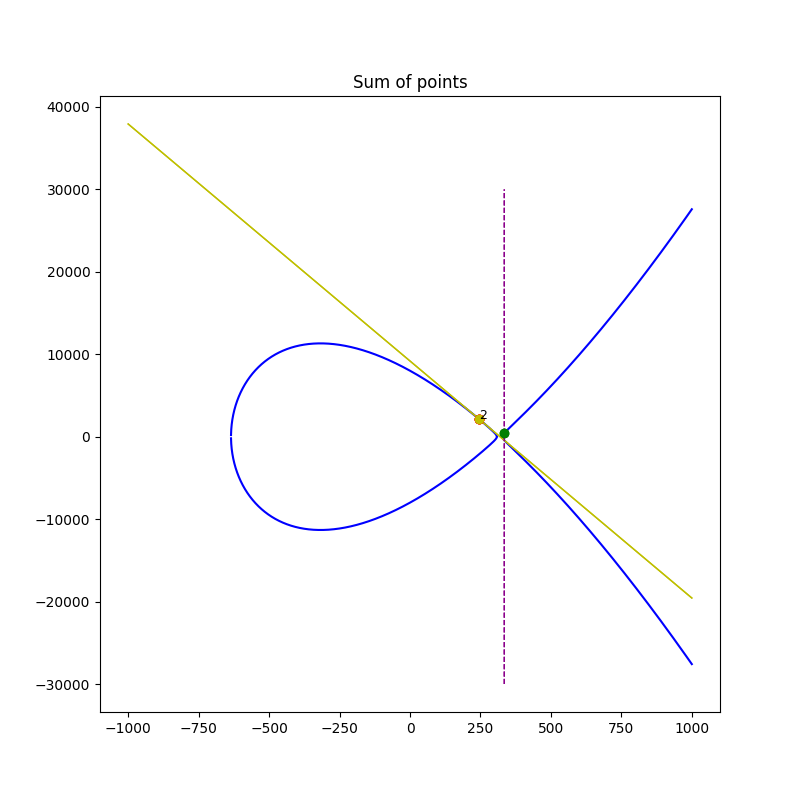
\includegraphics[width = 5cm]{../images/sum1.png}
    				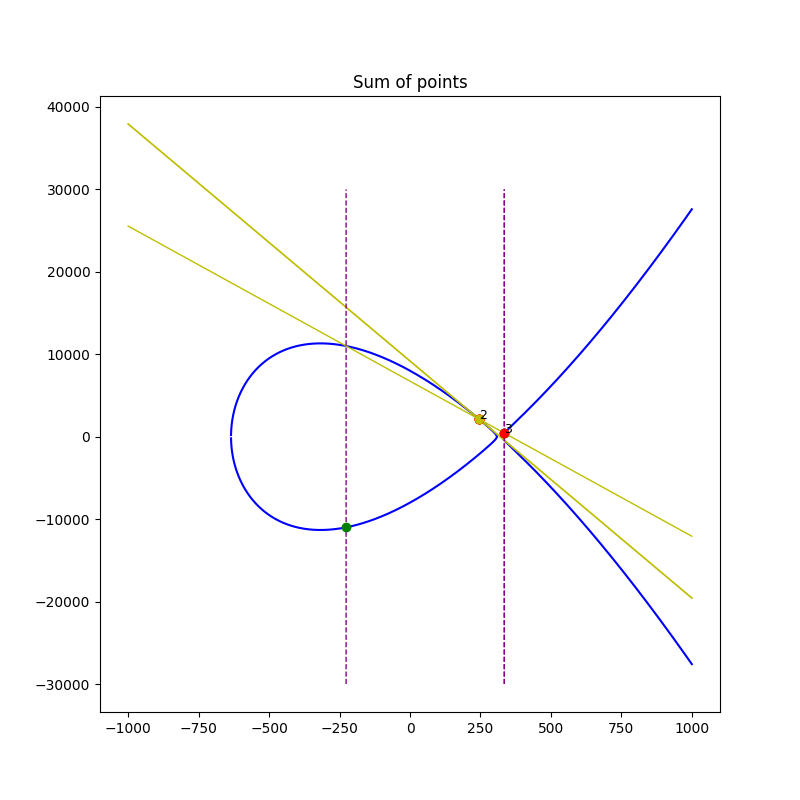
\includegraphics[width = 5cm]{../images/sum2.png}
    			\end{figure}
    	 	\end{block}

    	}
	\end{frame}
	
	\begin{frame}
		\onslide<+->{
			\begin{block}{Наглядное умножение на скаляр в исходной задаче}
				\begin{figure}[H]
					
					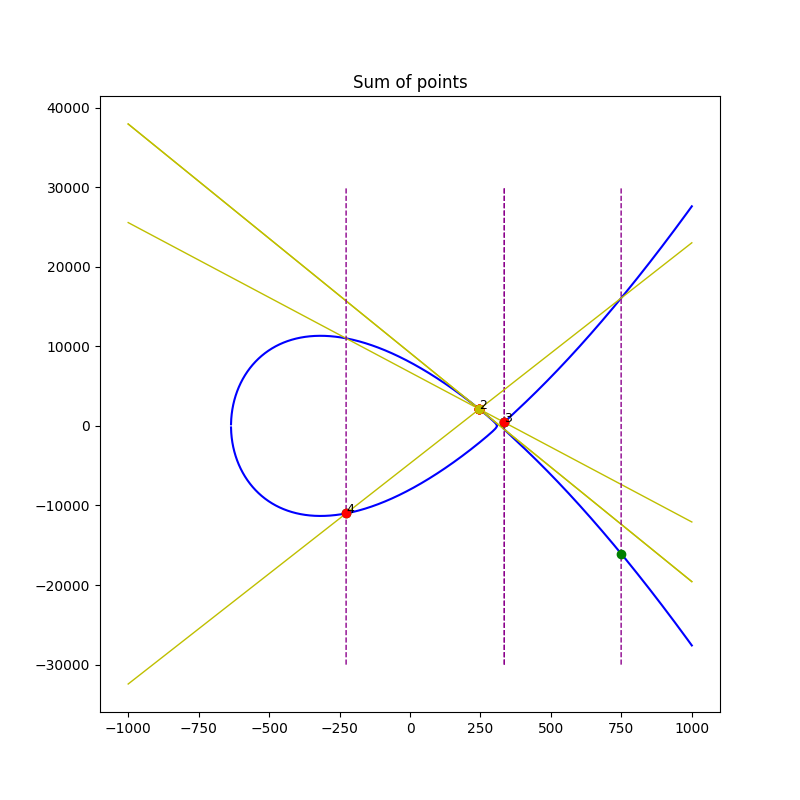
\includegraphics[width = 5cm]{../images/sum3.png}
					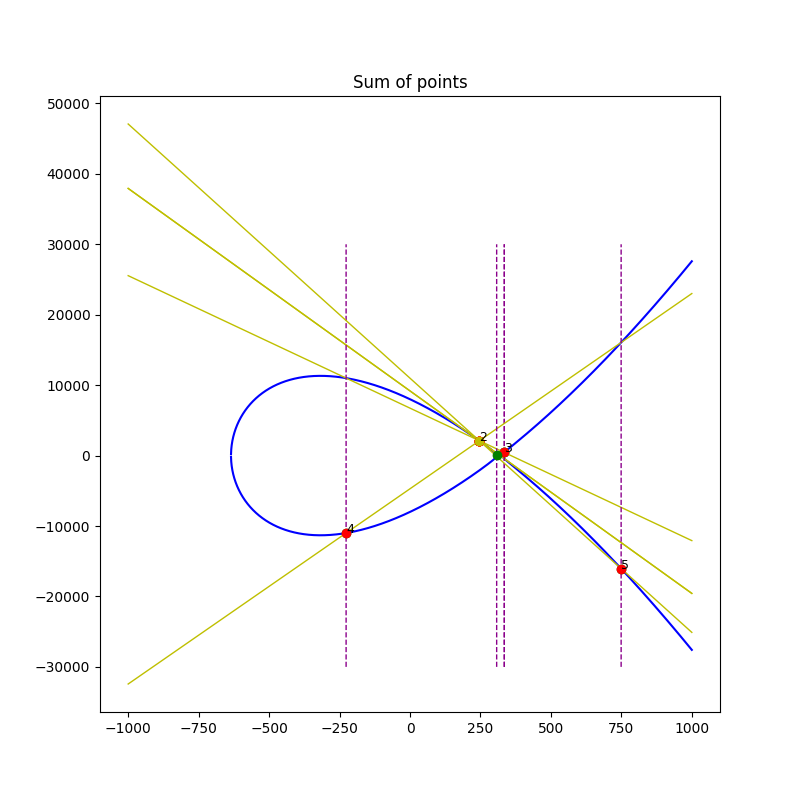
\includegraphics[width = 5cm]{../images/sum4.png}
				\end{figure}
			\end{block}
			
		}
	\end{frame}
	
	\begin{frame}
		\onslide<+->{
			\begin{block}{Финальная картинка}
				\begin{figure}[H]
					
					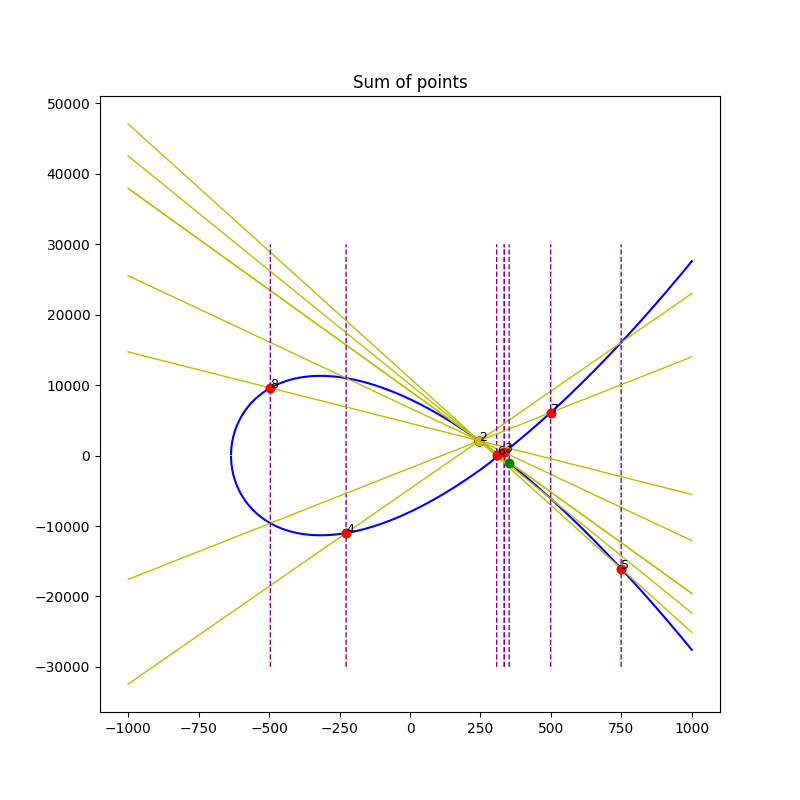
\includegraphics[width = 9cm]{../images/sum6.png}
		
				\end{figure}
			\end{block}
			
		}
	\end{frame}
	
	
	\begin{frame}
		\onslide<+->{
			\begin{block}{}
				Теперь у нас все готово для решения первоначальной задачи.
				Дадим краткое описания алгоритма, который был реализован.
			\end{block}
			\begin{block}{Алгоритм. Шаг 1.}
				Программа приводит кубику
				 \[
				x^3 + y^3 + z^3 + (1 - N) (x^2 y + y^2 x + x^2 z + z^2 x + y^2 z + z^2 y)
				+ (3 - 2 N) x y z = 0 \qquad (*)
				.\]  
				к нормальной форме Вейештрасса. То есть находит коэффициенты a, b
				и прямое и обратное преобразование.
				
			\end{block}
		
					\begin{block}{Замечание}
					Хоть для кубик вида $(*)$ известны явные формолы для коэффициентов $a, b$, а так же для преобразования в терминах $N$, программа проделывает это вычисления отдельно. Это позволяет применить этот алгоритм почти для произвольной кубики. 
				
					\end{block}
		
		
			
		}
	\end{frame}

	\begin{frame}
		\onslide<+->{
			\begin{block}{Алгоритм. Шаг 2.}
				На кубике находится произвольная рациональная точка \(P \notin \mathrm{Tor} \, (E(\QQ)) \). Это выполняется простым перебором числа $x = \frac{p}{q}$ где $p, q$ ищутся в определенных пределах.
		
			\end{block}
		
			\begin{block}{Алгоритм. Шаг 3.}
				Далее найденная точка умножается на себя $n$ раз. Именно поэтому важно, чтобы исходная точка не являлась точкой кручения.
				
			\end{block}
		
			\begin{block}{Алгоритм. Шаг 4.}
				Находятся координаты точек в изначальной системе. Отбираются точки у которых все координаты одного знака. 
			
			
			\end{block}
		
	
	}	
	\end{frame}

	\begin{frame}
		\onslide<+->{

			\begin{block}{Алгоритм. Итог}
				В случае исходной задачи
	            \[
				\frac{x}{y + z}  + \frac{y}{x + z} + \frac{z}{x + y} = 4,
				\qquad x, y, z \in \NN
				.\]
				При удачном выборе  $P$, точка  $9P$ будет соответсвовать решению уравнения. В котором будет порядка 80 цифр.

		
			\end{block}
		
		
			}
		\end{frame}
	

	
	




\end{document}
